\documentclass{standalone}
\usepackage{graphicx}	
\usepackage{amssymb, amsmath}
\usepackage{color}

\usepackage{tikz}
\usetikzlibrary{intersections, backgrounds, math}
\usepackage{pgfmath}

\definecolor{light}{RGB}{220, 188, 188}
\definecolor{mid}{RGB}{185, 124, 124}
\definecolor{dark}{RGB}{143, 39, 39}
\definecolor{highlight}{RGB}{180, 31, 180}
\definecolor{light_teal}{RGB}{107, 142, 142}
\definecolor{mid_teal}{RGB}{72, 117, 117}
\definecolor{dark_teal}{RGB}{29, 79, 79}
\definecolor{gray10}{gray}{0.1}
\definecolor{gray20}{gray}{0.2}
\definecolor{gray30}{gray}{0.3}
\definecolor{gray40}{gray}{0.4}
\definecolor{gray60}{gray}{0.6}
\definecolor{gray70}{gray}{0.7}
\definecolor{gray80}{gray}{0.8}
\definecolor{gray90}{gray}{0.9}
\definecolor{gray95}{gray}{0.95}

\begin{document}

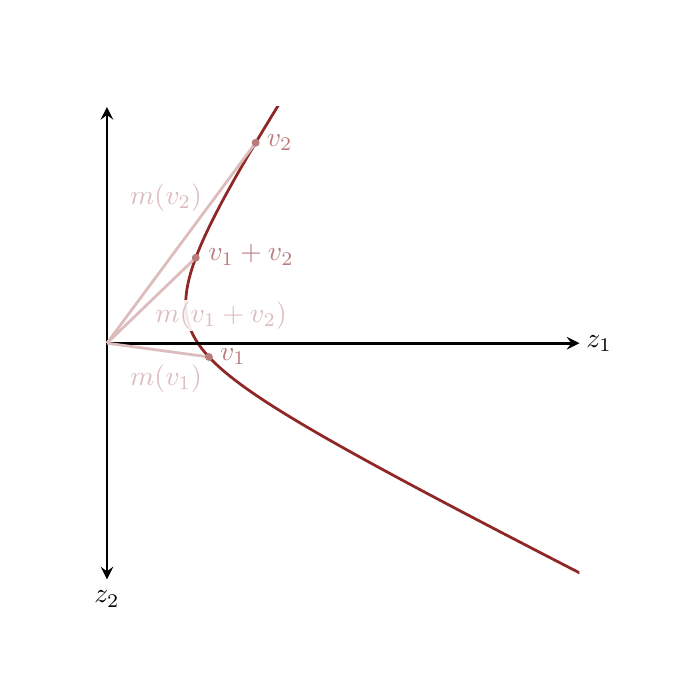
\begin{tikzpicture}[scale=1.0]
  \draw[white] (-1, -4) rectangle (7, 4);
   
  \pgfmathsetmacro{\a}{-0.5}
  \pgfmathsetmacro{\b}{1.5}
 
  \begin{scope}
    \clip (0, -3) rectangle (6, 3);

    \draw[domain={-3:2}, smooth, samples=50, line width=1.0, variable=\z, color=dark] 
      plot ({cosh(\z)}, {0.5 * (\b - \a) * sinh(\z) + 0.5 * (\b + \a) * cosh(\z)});
  \end{scope}

  \draw[<->, >=stealth, line width=1] (0, -3) -- (0, 3);
  \node at (0, -3.25) { $z_{2}$ };
  \draw[->, >=stealth, line width=1] (0, 0) -- (6, 0);
  \node at (6.25, 0) { $z_{1}$ };
  
  \pgfmathsetmacro{\z}{-0.75}
  \draw[light, line width=1] (0, 0) -- ({cosh(\z)}, {0.5 * (\b - \a) * sinh(\z) + 0.5 * (\b + \a) * cosh(\z)});
  \fill[mid] ({cosh(\z)}, {0.5 * (\b - \a) * sinh(\z) + 0.5 * (\b + \a) * cosh(\z)}) circle (0.05)
  node[right, xshift=0.5, yshift=0.0] { $v_{1}$ }; 
  
  \pgfmathsetmacro{\z}{1.25}
  \draw[light, line width=1] (0, 0) -- ({cosh(\z)}, {0.5 * (\b - \a) * sinh(\z) + 0.5 * (\b + \a) * cosh(\z)});
  \fill[mid] ({cosh(\z)}, {0.5 * (\b - \a) * sinh(\z) + 0.5 * (\b + \a) * cosh(\z)}) circle (0.05)
  node[right, xshift=0.5] { $v_{2}$ }; 
  
  \pgfmathsetmacro{\z}{0.5}
  \draw[light, line width=1] (0, 0) -- ({cosh(\z)}, {0.5 * (\b - \a) * sinh(\z) + 0.5 * (\b + \a) * cosh(\z)});
  \fill[mid] ({cosh(\z)}, {0.5 * (\b - \a) * sinh(\z) + 0.5 * (\b + \a) * cosh(\z)}) circle (0.05)
  node[right, xshift=1, yshift=1] { $v_{1} + v_{2}$ };
  
  \node[light] at (0.75, 1.85) { $m(v_{2})$ };
  \node[light] at (0.75, -0.45) { $m(v_{1})$ };
  \fill[white, opacity=0.9] (0.6, 0.15) rectangle (2.3, 0.55);
  \node[light] at (1.45, 0.35) { $m(v_{1} + v_{2})$ };
\end{tikzpicture}

\end{document}  